\chapter{Fundamentação Teórico-metodológica}

Em cada célula dos organismos vivos, para que ocorra a transcrição de um gene é necessário a ação conjunta dos fatores de transcrição e dos elementos regulatórios. Os fatores de transcrição são proteínas que se ligam nos elementos regulatórios. Já os elementos regulatórios são pequenos segmentos de DNA localizados em uma região antes do gene que será transcrito. Essa região é chamada de região promotora (ou reguladora), na figura \ref{fig:promotores_noDNA}, podemos observar a região promotora e os elementos regulatórios, onde os fatores de transcrição se conectarão.

\begin{figure}[htb!]
    \centering
    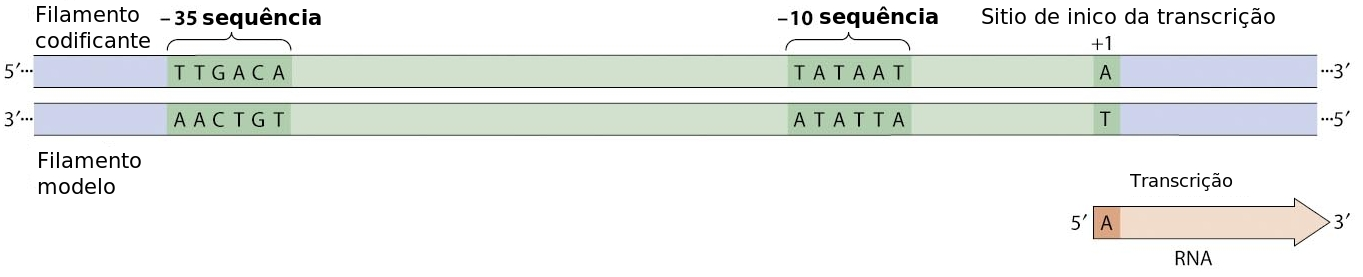
\includegraphics[scale=0.7]{./imagens/promotores_noDNA.jpg}
    \caption{Região promotora}
    \label{fig:promotores_noDNA}
\end{figure}

É de grande importância a identificação dos elementos regulatórios. Uma vez que eles estão ligados com a expressão de um gene. O conhecimento agregado com a identificação desses elementos pode levar a melhoramentos genéticos de organismos importantes para o consumo e a economia mundial, como por exemplo de grãos como o arroz, soja e milho.

No empenho de encontrar elementos regulatórios diversos algoritmos foram propostos. Das e Dai \cite{Das2007} os classificaram em três grupos:

\begin{itemize}
\item Os baseados em sequências promotoras de genes que são regulados pelos mesmos fatores de transcrição (genes co-regulados); estes métodos se concentram em apenas um único genoma.
\subitem Este ainda é subdividido em : predição probabilistica e predição baseada em palavras.

\item Os que utilizam sequências promotoras de genes ortólogos, que são sequências de DNA similares a várias espécies, indicando que estas espécies derivaram de um ancestral comum, também chamados de métodos de rastros filogenéticos.

\item Os métodos que combinam rastros filogenéticos e sequências promotoras de genes co-regulados.
\end{itemize}

Esses algoritmos utilizam de sequências de DNA como entrada. A sequência de DNA é formada pelo alfabeto (A, C, G e T). Cada letra representa uma base nitrogenada no DNA, que formará extensas palavras sem nenhuma restrição de posições. Para que possa ser manipulada no computador essas sequências são geralmente representadas por arquivos texto com a extensão \textit{.fasta} (figura \ref{fig:exe_seq}).

\begin{figure}[htb!]
    \centering
    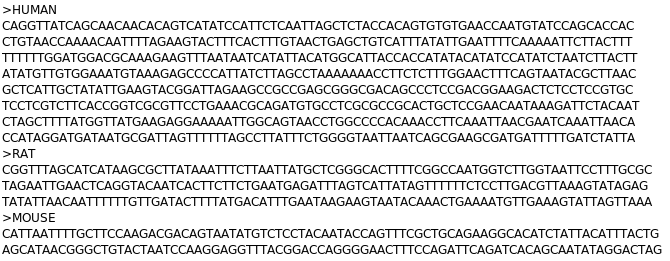
\includegraphics[scale=0.7]{./imagens/exe_seq.png}
    \caption{Exemplo de um arquivo de sequência de DNA}
    \label{fig:exe_seq}
\end{figure}

Esses arquivos de sequência de DNA podem ser encontrados embancos de dados públicos como SoyDB, Phytozome e o TRANSFAC.

Dentro dessas sequências, estão os elementos regulatórios (figura \ref{fig:exe_elemen}). Mas diversos fatores como, a remoção e a mutação de uma base e talvez o principal: a não padronização dos elementos regulatórios, tornam difícil a sua identificação.

\begin{figure}[htb!]
    \centering
    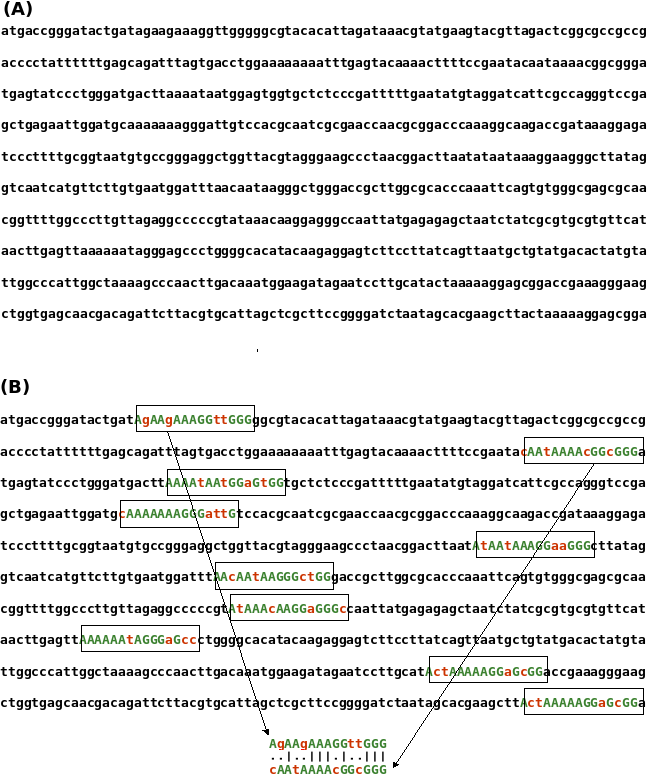
\includegraphics[scale=0.7]{./imagens/exe_element.png}
    \caption{(A)Sequência regulatória (B)Elementos regulatórios identificados}
    \label{fig:exe_elemen}
\end{figure}

\section{Algoritmos de predição de elementos regulatórios}

Apesar dos avanços para encontrar elementos regulatórios, a busca \textit{in silico} não é tão precisa quanto, por exemplo, a classificação de genes, gerando muitos resultados falsos. Isto deixa em aberto um vasto campo para ser explorado \cite{Rombauts2003}. Nos parágrafos a seguir serão discutidos alguns algoritmos.

Para identificar os elementos regulatórios em leveduras (\textit{Saccharomyces cerevisiae}) \cite{Helden1998}, propuseram o Oligo-Analysis, um algoritmo baseado na predição em palavras. Neste algoritmo foram usadas sequências promotoras de genes co-regulados, e para a identificação dos elementos foi utilizado o método de enumeração exaustiva, que computa todas as possíveis subsequências possíveis através das sequências promotoras.

Blanchette \textit{et al.} \cite{Blanchette2002}, utilizaram da abordagem de predição baseada em rastros filogenéticos, para desenvolver o FootPrinter. Assim como todos os outros algoritmos que se baseiam nessa abordagem, eles assumem que os elementos regulatórios são regiões conservadas que não sofreram muitas mutações ao longo da evolução. Este algoritmo tem como entrada as sequências promotoras de várias espécies e a árvore filogenética das espécies relacionadas. As sequências de cada espécie são inseridas nas folhas da árvore, então são feitas varias comparações das sequências, a começar das folhas. As sequências de tamanho \textit{k}, mais conservadas são promovidas para o nível acima da árvore, são feitas novas comparações até ser atingido a raiz da árvore, chegando a sequências ótimas, que passarão por mais comparações, desta vez da raiz até as folhas, finalizando o algoritmo com os elementos preditos.

Sinha \textit{et al.} \cite{Sinha2004}, propuseram um algoritmo combinando as técnicas probabilísticas e de rastros filogenéticos. O algoritmo permite a entrada de sequências promotoras de genes ortólogos, relacionadas com a árvore filogenética definida pelo usuário. As sequências dos elementos regulatórios podem ser conservadas ou não conservadas, o algoritmo as trata de maneira diferente. O algoritmo permite uma flexibilidade, na escolha da árvore filogenética, podendo escolher espécies distantemente relacionadas, que além da identificação dos elementos conservados entre as espécies possibilita a identificação de elementos que não estão relacionados com as espécies ortólogas.